\documentclass{article}

\usepackage[preprint]{neurips_2026}

\usepackage[utf8]{inputenc}
\usepackage[T1]{fontenc}
\usepackage{hyperref}
\usepackage{url}
\usepackage{booktabs}
\usepackage{amsfonts}
\usepackage{nicefrac}
\usepackage{microtype}
\usepackage{xcolor}
\usepackage{tikz}

\title{Instagram Reel Virality Probability}

\author{%
  Iban Rosales
  \And
  Ethan Fang
  \And
  Conner Satawidinata
  \And
  Benjamin Miller
}

\begin{document}

\maketitle

\section{Problem Description}
  In the past decade social media has become one of the greatest drivers of culture.
  What goes viral on social media is highly impactful to society and what is popular.
  Instagram is one of the largest of the social media platforms, making it one of the
  most influential drivers of culture. In the past decade, vertical short-form video
  platforms, such as Instagram Reels, have become one of the most popular ways of
  consuming social media content. Being able to go viral on social media is by extension
  the ability to shape culture. This is why it is important to determine which
  characteristics of an Instagram Reel are most associated with virality, and how does
  observing these characteristics change the probability that a Reel is viral? This is
  important because it shapes generations' culture and shows what is valued in our
  society.

\section{Data Sourcing and Processing}

\subsection{Data Source}
We used
\href{https://www.kaggle.com/datasets/deepeshkansotia/what-makes-an-instagram-reel-go-viral/data}{\textcolor{blue}{What Makes an Instagram Reel Go Viral Dataset}}
from Kaggle.
This dataset includes 100,000 synthetic samples based on real data and 26 features including posting
time, video length, virality score, and more.


\subsection{Preprocessing}
We found the data set was clean 

\textit{[TODO: Describe missing-data handling, feature selection, discretization
thresholds, and data splits. Explain why each processing step is needed.]}

\section{Modeling and Inference}

\subsection{Model Structure and Assumptions}
With said 7 most relevant features we will make a Bayesian Network using that subset of
the 26 features.

\begin{figure}[t]
  \centering
  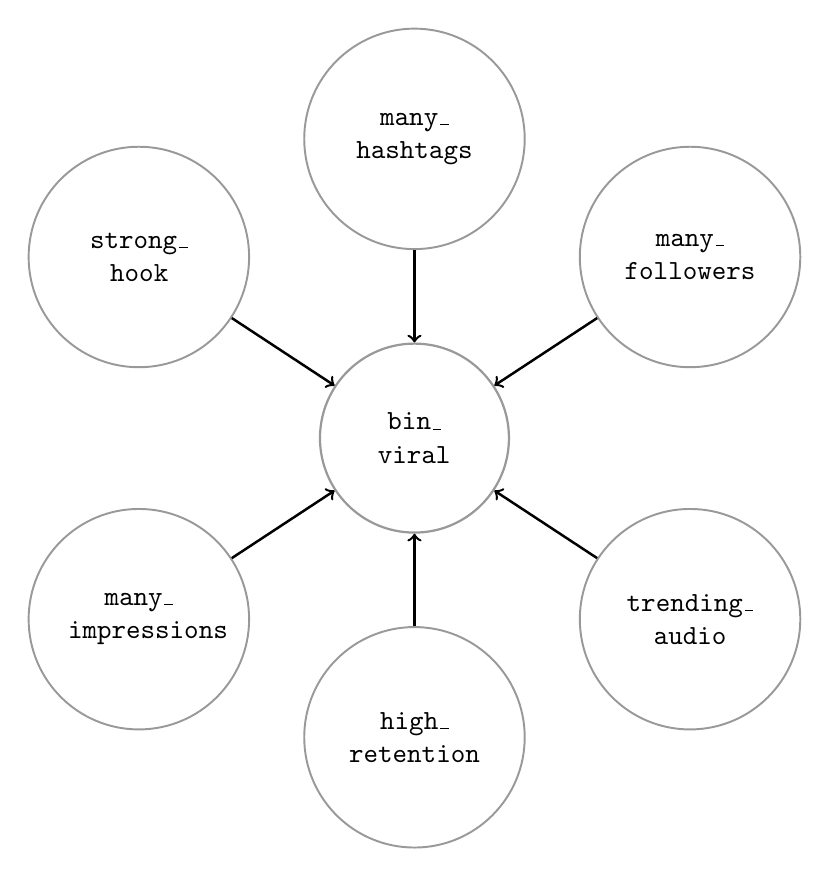
\begin{tikzpicture}[
    feature/.style={
      circle,
      draw=gray!80,
      line width=0.7pt,
      minimum width=2.8cm,
      minimum height=2.8cm,
      text width=1.8cm,
      align=center,
      inner sep=2pt
    },
    target/.style={
      circle,
      draw=gray!80,
      line width=0.8pt,
      minimum width=2.4cm,
      minimum height=2.4cm,
      text width=1.6cm,
      align=center,
      inner sep=2pt
    },
    edge/.style={
      ->,
      black,
      line width=0.9pt
    }
  ]
    \node[feature] (hook) at (-3.5, 2.3)
      {\texttt{strong\_}\\\texttt{hook}};
    \node[feature] (hashtags) at (0, 3.8)
      {\texttt{many\_}\\\texttt{hashtags}};
    \node[feature] (followers) at (3.5, 2.3)
      {\texttt{many\_}\\\texttt{followers}};
    \node[feature] (audio) at (3.5, -2.3)
      {\texttt{trending\_}\\\texttt{audio}};
    \node[feature] (retention) at (0, -3.8)
      {\texttt{high\_}\\\texttt{retention}};
    \node[feature] (impressions) at (-3.5, -2.3)
      {\texttt{many\_}\\\texttt{impressions}};

    \node[target] (viral) at (0, 0)
      {\texttt{bin\_}\\\texttt{viral}};

    \draw[edge] (hook) -- (viral);
    \draw[edge] (hashtags) -- (viral);
    \draw[edge] (followers) -- (viral);
    \draw[edge] (audio) -- (viral);
    \draw[edge] (retention) -- (viral);
    \draw[edge] (impressions) -- (viral);
  \end{tikzpicture}
  \caption{Bayesian network with binarized Reel features as predictors of the
  binary virality target.}
  \label{fig:bayesian-network}
\end{figure}

The network contains six binary predictor variables:
\texttt{strong\_hook}, \texttt{many\_hashtags},
\texttt{many\_impressions}, \texttt{many\_followers},
\texttt{trending\_audio}, and \texttt{high\_retention}.
The target variable is \texttt{bin\_viral}, which is 1 when
\texttt{virality\_score} is at or above its 99.5th percentile and 0
otherwise. The notebook binarizes each continuous predictor at its
median; \texttt{trending\_audio} is encoded as 1 for true and 0 for
false.

As shown in Figure~\ref{fig:bayesian-network}, each predictor has a
directed edge to \texttt{bin\_viral}, and there are no edges between
predictors. Let $X_1,\ldots,X_6$ denote the predictor variables and let
$Y$ denote \texttt{bin\_viral}. The joint distribution represented by
this structure factorizes as
\[
P(X_1,\ldots,X_6,Y)
=
\left(\prod_{i=1}^{6} P(X_i)\right)
P(Y\mid X_1,\ldots,X_6).
\]
Thus, the model estimates the probability of the binary virality outcome
given the observed feature values. The structure assumes that the
predictors are marginally independent; this is a simplifying assumption
that may not hold for correlated features. The arrows describe the
network's assumed dependencies and do not imply causal relationships.

We will estimate each root variable's probability table from its
observed category frequencies in the training data. The conditional
probability table for \texttt{bin\_viral} would have $2^6=64$ rows, one for each
combination of predictor values. For each row, the probability of each
target value is estimated from the relative frequency of that value among
training examples with the corresponding predictor combination. The
notebook currently performs the binarization but does not yet estimate
these probability tables.

\subsection{Inference Algorithm}
We intend to use approximate inference to estimate the probability that a Reel is
viral given observed characteristics.

\textit{[TODO: Specify the implemented inference algorithm, evidence and query
variables, algorithm settings, and implementation details.]}

\section{Results and Discussion}

\subsection{Experimental Configurations}
\textit{[TODO: Compare multiple configurations, such as inference settings,
feature subsets, discretization thresholds, or network structures. Describe the
evaluation procedure and explain observed performance differences.]}

\subsection{Quantitative Results}
\textit{[TODO: Report measured results with suitable metrics, tables, or figures.
Explain the metrics and compare performance across configurations.]}

\subsection{Qualitative Insights}
\textit{[TODO: Explain what the model captures about the data, how observing
features changes virality probabilities, and whether learned conditional
probability tables align with intuition.]}

\subsection{Convergence and Scalability}
\textit{[TODO: Discuss training or inference stability, convergence, runtime,
and computational cost as the dataset or network grows.]}

\section{Conclusion}
\textit{[TODO: Summarize key findings and model performance. Discuss limitations,
including the use of synthetic data, and propose extensions or improvements.]}

\section{Reflections \& Contributions}

\subsection{Advice for Future Students}
\textit{[TODO: Share practical suggestions and lessons learned from the project.]}

\subsection{Individual Contributions and Reflections}
\paragraph{Iban Rosales}
\textit{[TODO: Write 1--2 sentences describing your contributions and a brief
individual reflection on the project.]}

\paragraph{Ethan Fang}
\textit{[Writing latex for the project report.]}

\paragraph{Conner Satawidinata}
\textit{[TODO: Write 1--2 sentences describing your contributions and a brief
individual reflection on the project.]}

\paragraph{Benjamin Miller}
\textit{[TODO: Write 1--2 sentences describing your contributions and a brief
individual reflection on the project.]}

\subsection{Use of Generative AI}
\textit{[TODO: Describe how generative AI was used in the project and how its
outputs were checked.]}

\section{References}
\textit{[TODO: Cite all external papers, datasets, and tools used in the project.
Replace this placeholder with the actual reference entries.]}

\end{document}
